%!TEX root = ../presentation.tex


\section{Teamarbeit}

\subsection{Kommunikation}
\begin{frame}{Kommunikation}
    \begin{itemize}
        \item Matrix (Element)
        \item Treffen am Montag
        \item GitHub Issues
    \end{itemize}
\end{frame}

\subsection{Anfangsstruktur}
\begin{frame}{Anfangsstruktur}
    \begin{figure}
        \centering
        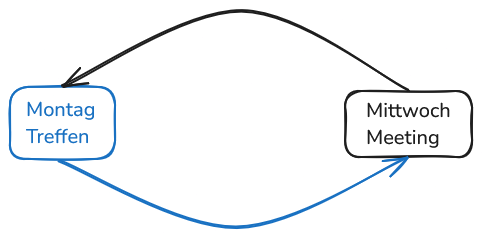
\includegraphics[width=0.6\linewidth]{pictures/level1}
        \label{fig:lvl1}
    \end{figure}
\end{frame}

\begin{frame}{Problem: Programmieren beim Montag Treffen}
    \begin{figure}
        \centering
        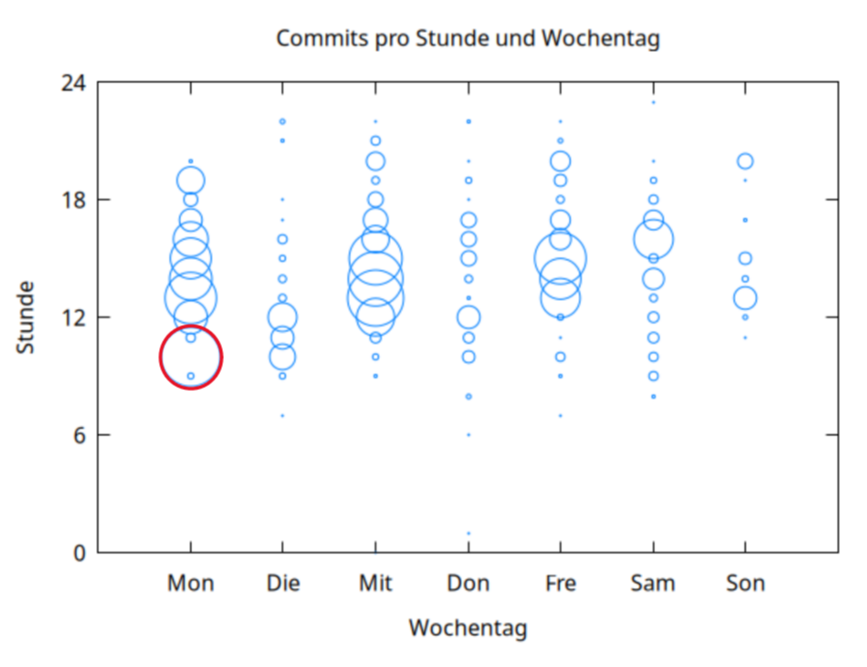
\includegraphics[width=0.52\linewidth]{pictures/hours}
        \label{fig:commit-hours}
    \end{figure}
\end{frame}

\subsection{1. Verbesserung}
\begin{frame}{1. Verbesserung}
    \begin{figure}
        \centering
        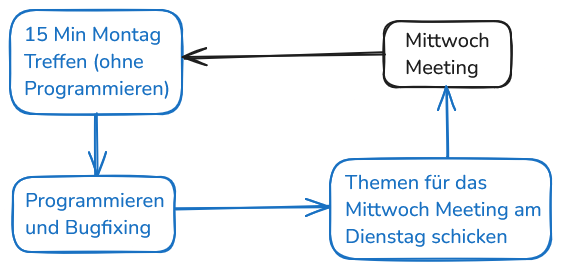
\includegraphics[width=0.6\linewidth]{pictures/level2}
        \label{fig:lvl2}
    \end{figure}
\end{frame}

\subsection{2. Verbesserung}
\begin{frame}{2. Verbesserung}
    \begin{figure}
        \centering
        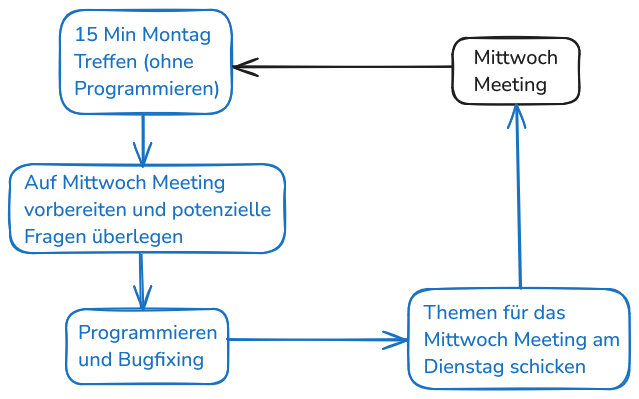
\includegraphics[width=0.6\linewidth]{pictures/level3}
        \label{fig:lvl3}
    \end{figure}
\end{frame}

\subsection{Wasserfallmodell}
\begin{frame}{Wasserfallmodell}
    \begin{itemize}
        \item Genutzt: Wasserfallmodell mit Rückkopplung
        \item Pros:
        \begin{itemize}
            \item Produktdefinition klar für alle
            \item Hohe Codequalität
        \end{itemize}
        \item Cons:
        \begin{itemize}
            \item Dokumentation aufwendig
            \item Rückkopplung nicht immer effizient
        \end{itemize}
    \end{itemize}
\end{frame}